\subsection{Velocity, the Speed of Light, and Causality} 

(Answers to M\Alph{subsection} problems are on page \pageref{velocities_causality_prob_answers}.)


\begin{Exercise}[difficulty=0]
In class, we derived the ``forward'' velocity transformation, in which we find the velocity $u'$ of an object in a new frame $S'$,
$$
%u'=\frac{u-v}{1-\dfrac{uv}{c^2}}.
u'=\frac{u-v}{1-({uv}/{c^2})}.
$$
In this problem, you will derive the ``reverse'' velocity transformation, in which the velocity $u$ of an object in the frame $S$ is expressed in terms of $u'$ and $v$.  You will do this in three different ways. (a)~Use algebraic manipulation to solve the equation above for u. (b)~Start with the ``reverse'' Lorentz transformations $x=\gamma(x'+vt')$ and $t=\gamma[t'+(v/c^2 )x']$, and follow similar logic to what we did in class.  (c)~Use the trick you described in Problem \ref{fourth_lorentz_derivation_prob}.
\end{Exercise}


\begin{Exercise}[difficulty=1]
Event A occurs at coordinates $(x,ct)=(4~{\rm m},6~{\rm m})$.  Event B occurs at coordinates $(7$~m$,11$~m). (a)~What is the numerical value of the spacetime interval $(\Delta s)^2$ between your two points?  (b)~Is the spacetime interval between these events \textit{timelike}, \textit{spacelike}, or \textit{lightlike}, and how do you know?  
\end{Exercise}
\begin{Answer}
(a) $-16$~m$^2$  (b) timelike.  (Why?) 
\end{Answer}


\begin{Exercise}[difficulty=1]
Event A occurs at coordinates $(x,ct)=(2 {\rm m},-3 {\rm m})$.  (a)~Find any point B such that the spacetime interval between points A and B is lightlike.  (b)~What is the numerical value of the spacetime interval $(\Delta s)^2$ between your two points?
\end{Exercise}
\begin{Answer}
(b) 0
\end{Answer}


\begin{Exercise}[difficulty=0]
Anna, Bob, and their roommate Carlos are quarantined together in a small apartment, and they are starting to get on each other's nerves.  The space-time (Minkowski) diagram on the right shows three events that happen one afternoon, in the reference frame of their feckless cat, who is sleeping on the sofa.  The dotted lines on the graph represent the speed of light, as usual.

\begin{minipage}{0.55 \textwidth}
\begin{itemize}[nosep]
\item At point A, Anna hiccups.  
\item At point B, Bob emits a sudden snorting noise. 
\item At point C, Carlos spills his drink on his lap.  
\item Carlos says, ``Darn it, Bob, you made me spill my drink!''
\item Bob says, ``Sorry Carlos, but I only snorted because Anna startled me when she hiccupped.''
\end{itemize}

\bigskip

\begin{enumerate}[nosep,label=(\alph*),series=mylist]
\item Could Bob snorting have caused Carlos to spill his drink?  Explain.
\item Could Anna hiccupping have caused Bob to snort? Explain.
\end{enumerate}
\end{minipage}
\begin{minipage}{0.44 \textwidth}
\hspace{\fill}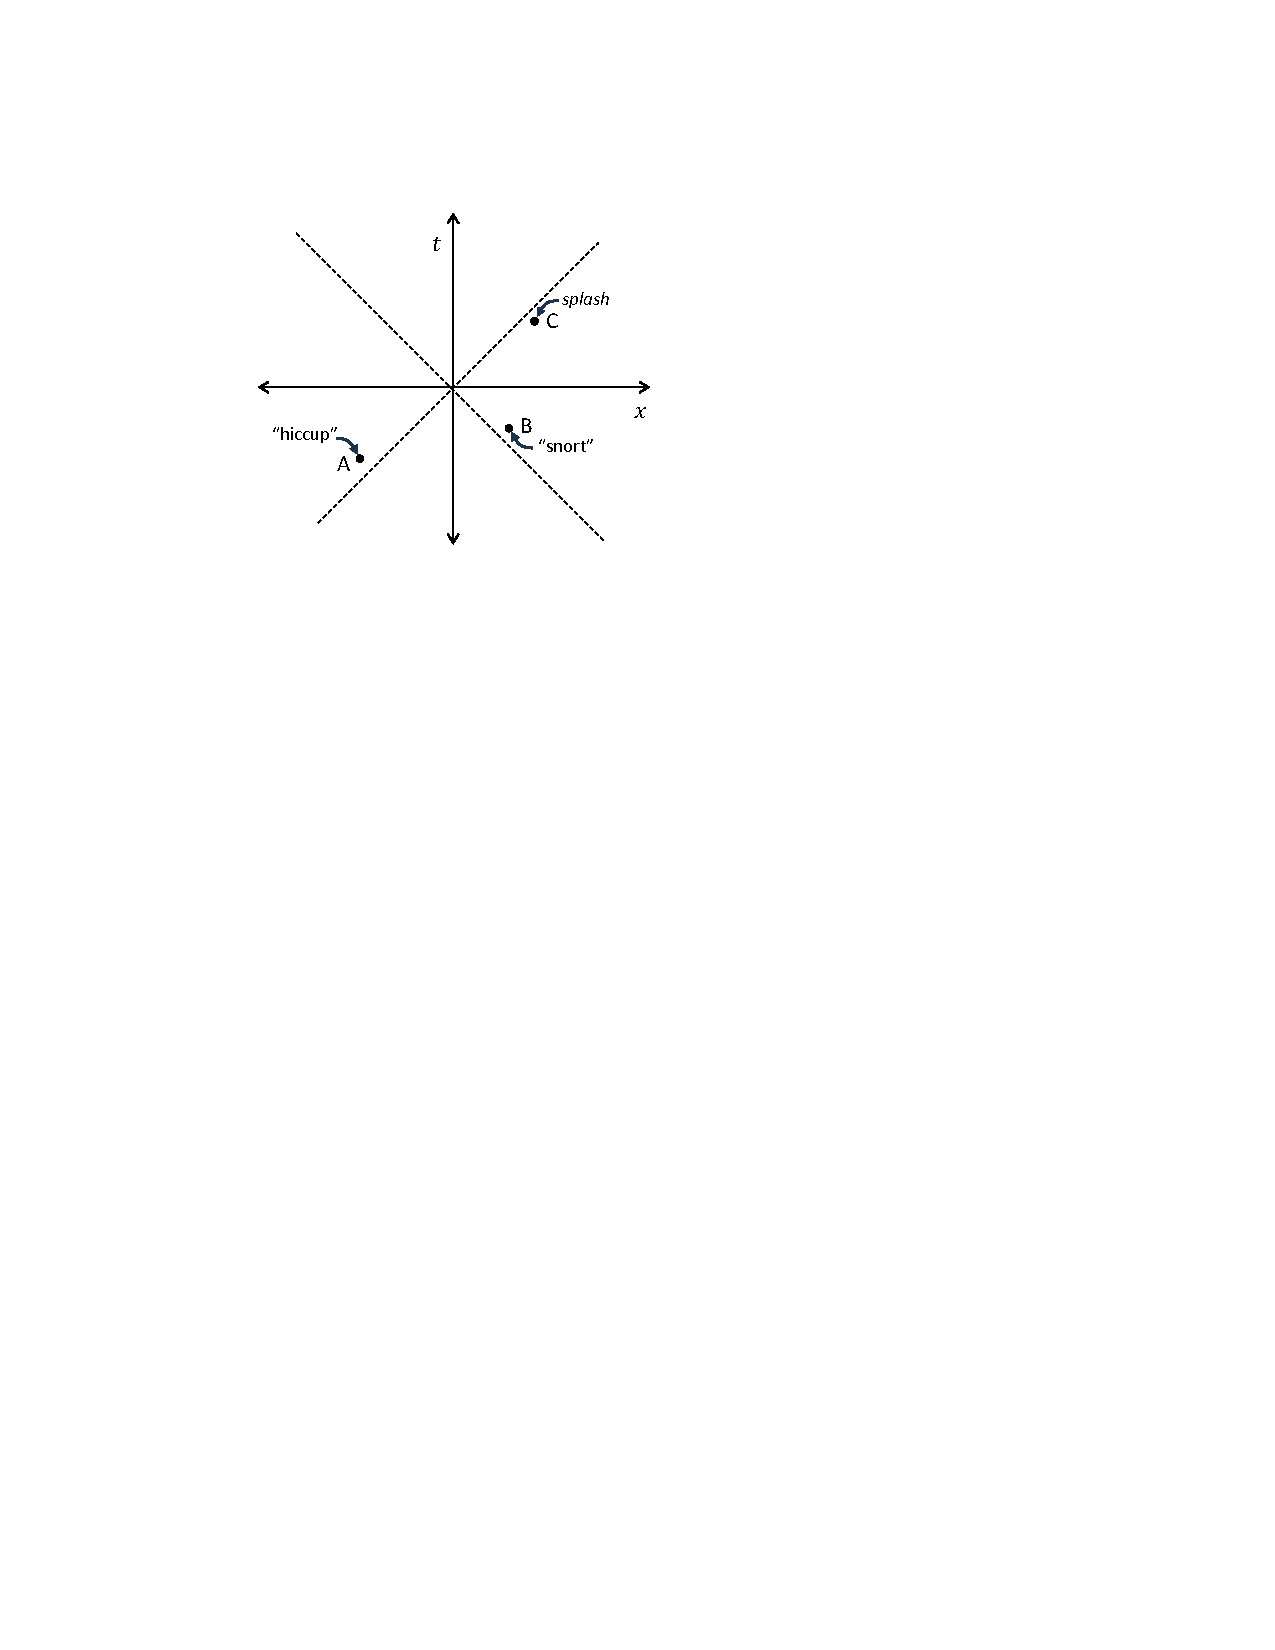
\includegraphics{M_problems/velocities_causality/hiccup_snort_splash.pdf}

\end{minipage}
\textit{Anna says, ``You are so full of it, Bob!  In case you didn't notice, I was traveling in the positive x-direction at a high velocity, and in my reference frame, you snorted before I hiccupped.  In fact, your snorting made me hiccup, so it's all your fault!''}
\begin{enumerate}[resume*=mylist] 
%There's a bug in enumitem that causes "resume" to fail when used in conjunction with minipage.  The fix is to use a named list (here "mylist").
\item Is it possible that Bob's snort happened before Anna's hiccup in Anna's reference frame? Explain.
\item Is it possible that Bob's snort caused Anna to hiccup?  Explain.
\end{enumerate}
\end{Exercise}
\begin{Answer}
(a) yes (b) no (c) yes (d) no
\end{Answer}


\begin{comment}
\begin{Exercise}[difficulty=1]
Two events occur at (x,ct) coordinates (4 m, 1 m) and (7 m, 6 m).  (a) Is the spacetime interval between these events timelike, spacelike, or lightlike?  (b) What is the proper time between these events?  (c) What is the proper distance between these two events?
\end{Exercise}
\begin{Answer}
MD6. (b) 4 m/c  (c) n/a
\end{Answer}



\begin{Exercise}[difficulty=1]
Two events occur at (x,ct) coordinates (-3 m, -2 m) and (7 m, 4 m).  (a) Is the spacetime interval between these events timelike, spacelike, or lightlike?  (b) What is the proper time between these events?  (c) What is the proper distance between these two events?
\end{Exercise}
\begin{Answer}
(a) spacelike (b) n/a (c) 8 m
\end{Answer}
\end{comment}




\bigskip\bigskip\bigskip
\pagebreak[3]
\textbf{Answers to Selected {\thesubsection} Problems:}
\label{velocities_causality_prob_answers}
%\shipoutExercise
\shipoutAnswer

\cleardoublepage